%Two improvements are proposed in this project: the mechanical stimulus from the fluid and the mass transfer from the fluid to the solid. Towards these ends, the overall framework must appropriately address these issues: (1) through the coupling of fluid and solid simulation, correctly identifying the mechanical stimuli applied to the solid growth, including both pressure and shear stress; (2) proposing reasonable assumptions on the mass flux, which is another essential impact on the growth process.

Considering the fluid environment and solid tissue as a system, the inputs to this system are the energy that drives the fluid flow and the mass source inside the tissue. What act as the bridge between the fluid and solid are the velocity, stress and mass flux. The velocity and stress coupling are general for all fluid-solid interaction problems, and have been taken care of by the IFEM formulation. Although mass flux interpolation is new, it is essentially a vector which should be identical on both the fluid and solid sides. Therefore the same interpolation functions as used on velocity can be applied to handle it.

With the presence of mass transfer, the mass equation needs to be modified. Recall the mass conservation of incompressible fluid states that the mass rate per unit volume is $0$, considering the mass flux, it is rewritten as:
\begin{equation}
\rho \nabla \cdot \bv = \nabla \cdot \bold{r}
\end{equation}
where $\bold{r}$ is the mass flux in the current configuration. 

Let us also exam the momentum equation. In our IFEM formulation, the fluid mesh is fixed. The existence of the solid is detected by the ``artificial fluid". As the solid increases in volume, the artificial fluid will also increase in volume, which automatically takes care of the real fluid momentum on its own. Therefore, the momentum equation remains unchanged.

%\subsubsection{Implementation}


Figure \ref{fig:framework} represents the overall framework. It can be seen that the solid growth is fully coupled with fluid environment. Following our previous work in \cite{Zhang, Zhang3, Zhang16, Zhang17}, the fluid and solid are solved individually on different meshes. The interface velocity and mass flux are distributed from the fluid to the solid and the volume force is distributed from the solid to the fluid. An initial disturbance is applied to the fluid, which generates the mechanical loads on the solid tissue and stimulates its growth.

\begin{figure}[H]
   \centering
   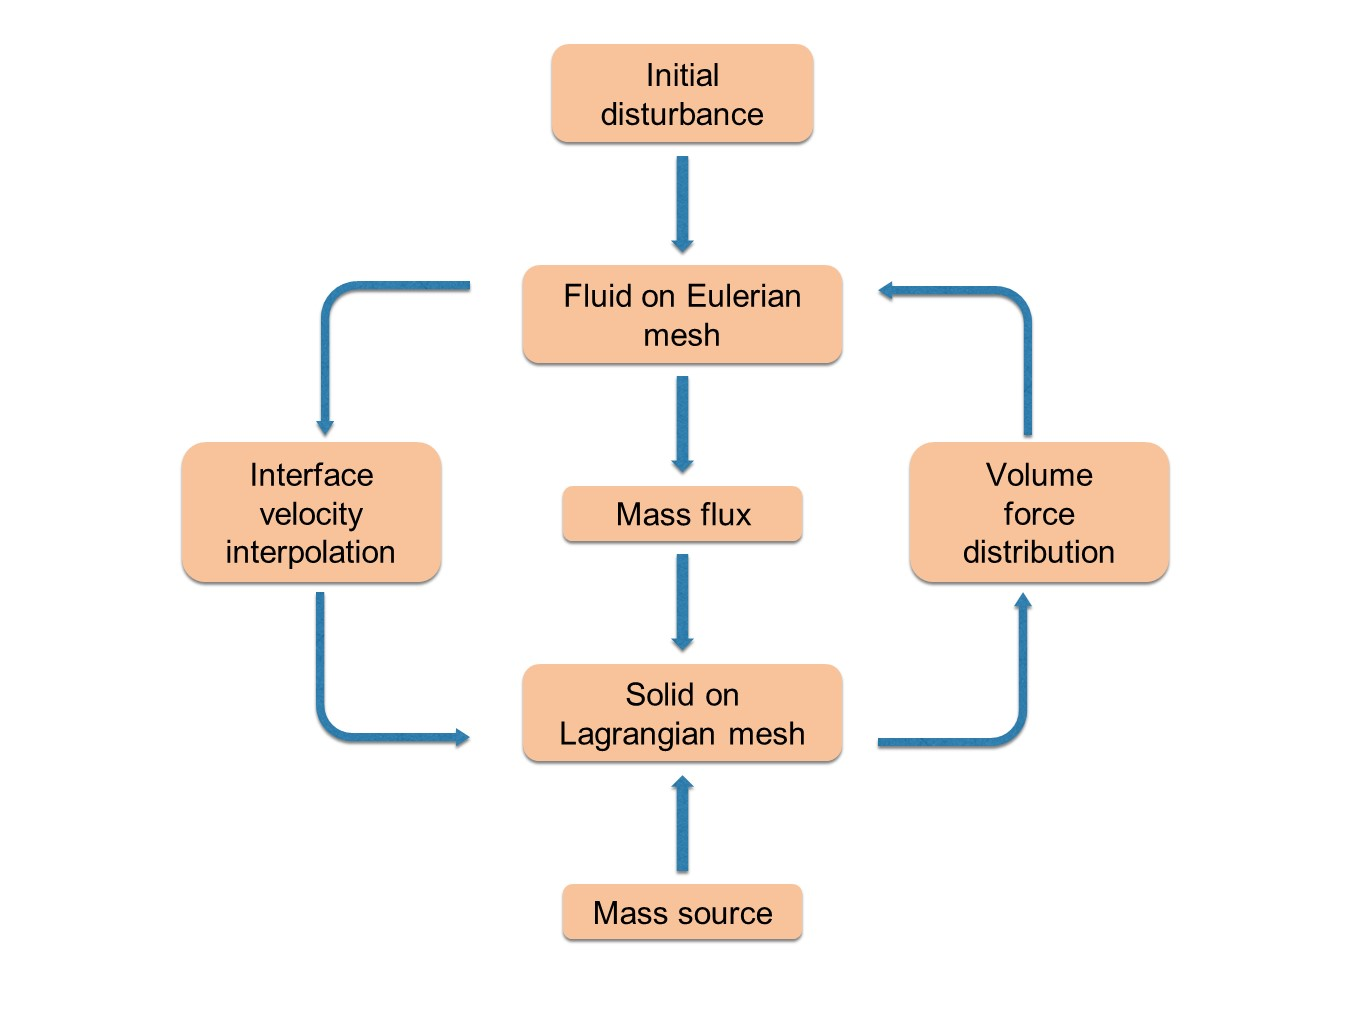
\includegraphics[width=.5\textwidth]{./figs/framework.jpg} % requires the graphicx package
   \caption{The numerical framework}
   \label{fig:framework}
\end{figure}





